%
% Niniejszy plik stanowi przykład formatowania pracy magisterskiej na
% Wydziale MIM UW.  Szkielet użytych poleceń można wykorzystywać do
% woli, np. formatujac wlasna prace.
%
% Zawartosc merytoryczna stanowi oryginalnosiagniecie
% naukowosciowe Marcina Wolinskiego.  Wszelkie prawa zastrzeżone.
%
% Copyright (c) 2001 by Marcin Woliński <M.Wolinski@gust.org.pl>
% Poprawki spowodowane zmianami przepisów - Marcin Szczuka, 1.10.2004
% Poprawki spowodowane zmianami przepisow i ujednolicenie
% - Seweryn Karłowicz, 05.05.2006
% Dodanie wielu autorów i tłumaczenia na angielski - Kuba Pochrybniak, 29.11.2016

% dodaj opcję [licencjacka] dla pracy licencjackiej
% dodaj opcję [en] dla wersji angielskiej (mogą być obie: [licencjacka,en])
\documentclass[licencjacka,en]{pracamgr}
\usepackage{hyperref}  % Enables clickable links
\usepackage{xcolor}    % Allows hyperlink color customization
\usepackage{graphicx}
\usepackage{listings}

% Define JSON formatting style for listings
\lstdefinelanguage{json}{
    basicstyle=\ttfamily\small,
    numbers=left,
    numberstyle=\tiny,
    stepnumber=1,
    showstringspaces=false,
    breaklines=true,
    frame=single,
    backgroundcolor=\color{gray!10},
    keywordstyle=\color{blue},
    stringstyle=\color{red}
}

% Set hyperlink colors
\hypersetup{
    colorlinks=false,
    urlcolor=blue
}

% Dane magistranta:
\autori{Szymon Kozłowski}{448304}
\autorii{Gustaw Blachowski}{448194}
\autoriii{Kamil Dybek}{448224}
\autoriv{Natalia Junkiert}{448267}

\title{Using machine learning models for processing the data presented to the user by mobile devices.}

\tytulang{Using machine learning models for processing data presented to user by mobile devices.}
\titlepl{Wykorzystanie modeli uczenia maszynowego do przetwarzania danych zaprezentowanych użytkownikowi przez urządzenie mobilne.}

%kierunek:
% - matematyka, informacyka, ...
% - Mathematics, Computer Science, ...
\kierunek{Computer Science}

% informatyka - nie okreslamy zakresu (opcja zakomentowana)
% matematyka - zakres moze pozostac nieokreslony,
% a jesli ma byc okreslony dla pracy mgr,
% to przyjmuje jedna z wartosci:
% {metod matematycznych w finansach}
% {metod matematycznych w ubezpieczeniach}
% {matematyki stosowanej}
% {nauczania matematyki}
% Dla pracy licencjackiej mamy natomiast
% mozliwosc wpisania takiej wartosci zakresu:
% {Jednoczesnych Studiow Ekonomiczno--Matematycznych}

% \zakres{Tu wpisac, jesli trzeba, jedna z opcji podanych wyzej}

% Praca wykonana pod kierunkiem:
% (podać tytuł/stopień imię i nazwisko opiekuna
% Instytut
% ew. Wydział ew. Uczelnia (jeżeli nie MIM UW))
\opiekun{Jacek Sroka PhD\\
  Institute of Informatics\\
  }

% miesiąc i~rok:
\date{\today}

%Podać dziedzinę wg klasyfikacji Socrates-Erasmus:
\dziedzina{ 
%11.0 Matematyka, Informatyka:\\ 
%11.1 Matematyka\\ 
%11.2 Statystyka\\ 
%11.3 Informatyka\\ 
11.4 Artificial Intelligence\\ 
%11.5 Nauki aktuarialne\\
%11.9 Inne nauki matematyczne i informatyczne
}

%Klasyfikacja tematyczna wedlug AMS (matematyka) lub ACM (informatyka)
\klasyfikacja{
  I.2.7: Natural Language Processing\\
  H.3.3: Information Search and Retrieval}

% Słowa kluczowe:
\keywords{LLM, NLP, BERT, Android, Edge-device, Fine-Tuning}

% Tu jest dobre miejsce na Twoje własne makra i~środowiska:
\newtheorem{defi}{Definicja}[section]

% koniec definicji

\let\cleardoublepage\clearpage
\begin{document}

\maketitle

%tu idzie streszczenie na strone poczatkowa
\begin{abstract}
In the era of rapidly evolving digital applications, traditional scraping techniques face increasing challenges in maintaining reliable data collection pipelines. Commissioned by Murmuras, a company specializing in commercial and scientific data analysis, in this project we present a novel approach to processing phone screen content, such as displayed social media posts and website advertisements. Our solution leverages Large Language Models (LLMs) running locally on the user's device to handle diverse data formats while ensuring that sensitive information remains protected. The primary application explored in this study is the extraction of discount coupons, demonstrating the feasibility of our method in identifying and structuring valuable content from varying digital sources. Furthermore, the system is designed to be easily adaptable to other use cases, such as analyzing users' political views. Additionally we explore usage of non-LLM models for the defined task. The results highlight the potential of LLM-driven content analysis as an alternative to conventional scraping techniques.
\raggedright
\end{abstract}

\tableofcontents
\listoffigures
\listoftables

\chapter{Introduction}

\section{Project background and motivation}
With the rapid advancement of information technology, the Internet has become one of the most crucial facets for many businesses to perform marketing activities\cite{design_of_coupons}. One of the key marketing tools in business-to-consumer (B2C) e-commerce is the digital coupon\cite{targeted_reminders}. Compared to paper coupons, digital coupons are characterized by their wide reach, rapid distribution, and low spread costs. Furthermore, a key advantage of digital coupons is their ability to facilitate targeted marketing by offering personalized discounts to different customers, thereby increasing sales\cite{design_of_coupons}.

Recent statistics underscore the significance of mobile devices in the domain of coupon distribution. For example, studies have shown that over 90\% of digital coupon users access their vouchers via smartphones\cite{emarketer_coupon_stats}, and similar figures are reported by other industry sources\cite{coupon_stats_2}. This high rate of mobile usage creates a pressing need for coupon analysis tools that are optimized for mobile platforms, ensuring that consumers receive timely and personalized offers regardless of their location or device.

Large Language Models (LLMs) have become a fundamental technique in contemporary machine learning, replacing previously utilized recurrent neural network (RNN) architectures in the field of natural language processing (NLP)\cite{li2024}. Subsequent research has demonstrated their applicability to structured input data\cite{sui2024}, such as screen views and coupons. Additionally, there have been efforts to integrate these models into web scraping pipelines\cite{scapegraph_repo}.

In light of these trends, the company Murmuras has tasked us with developing a solution based on a machine learning model that can be deployed as a mobile application. This model will process input representing the user's onscreen view and extract digital coupons along with their relevant data. This solution must be capable of running locally on the device, ensuring efficient processing without relying on external servers. By leveraging advanced machine learning techniques, the app will handle the diverse formats and layouts of digital coupons, thus facilitating the collection of data regarding coupons.

\section{The definition of a coupon}
A coupon is a physical piece of paper or digital voucher that can be redeemed for a financial discount when purchasing a product\cite{coupon_definition}. A coupon is characterized by a name, expiration date, and a discount type, e.g. '20\% off', 'buy 1 get 1 free', etc., however, not every coupon contains each of these features. Furthermore, coupons may contain numerous other features such as images and eligibility requirements. Henceforth, the term 'coupon' will refer exclusively to a digital coupon. The term 'conventional coupon' will refer to the traditional physical coupon. Examples of digital coupons encountered in mobile applications are presented in \ref{fig:example_coupons}

\begin{figure}[h]
    \centering
    \begin{minipage}{0.45\textwidth}
        \centering
        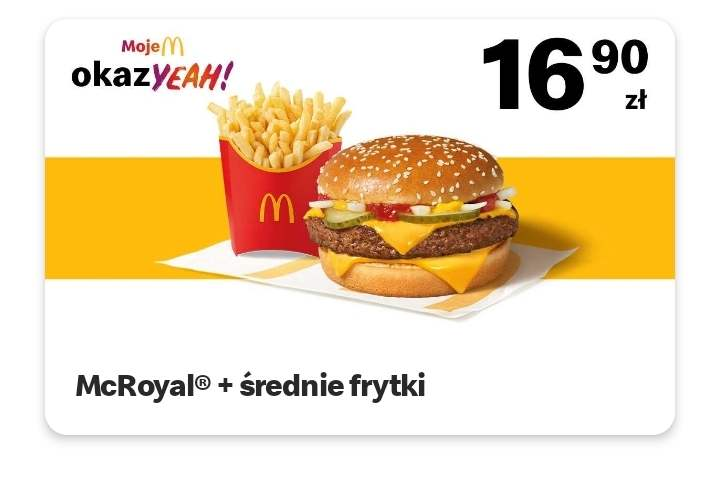
\includegraphics[width=\linewidth]{bachelor_images/coupon1.jpg}
        \caption{Example coupon from fast-food restaurants chain mobile application}
    \end{minipage}
    \hfill
    \begin{minipage}{0.45\textwidth}
        \centering
        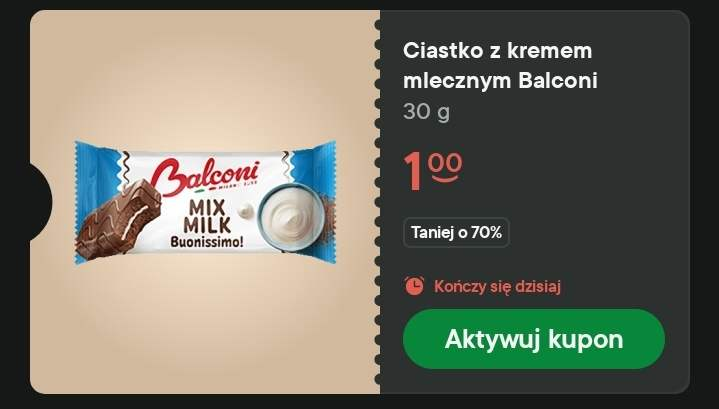
\includegraphics[width=\linewidth]{bachelor_images/coupon2.jpg}
        \caption{Example coupon from grocery store mobile application}
    \end{minipage}
    \caption{Example digital coupons}
    \label{fig:example_coupons}
\end{figure}


\subsection{Our data model of digital coupon}
\label{sec:coupon_model}
In the following research we model a digital coupon as a collection of named fields:
\begin{enumerate}
    \item \textit{product\_name}: the name of the product,
    \item \textit{valid\_until}: the text representing the date of coupon expiration,
    \item \textit{discount\_text}: the text representing the discount offered to the user,
    \item \textit{activated}: either true or false, indicates whether the coupon has been activated,
\end{enumerate}
We allow for special \textit{null} value in the above fields in case no data is available.

An example of a digital coupon represented in JSON format is shown in listing \ref{lst:coupon_example}:

\begin{lstlisting}[language=json, caption={Example of a digital coupon in JSON format}, label={lst:coupon_example}]
{
    "product_name": "Shampoo X",
    "valid_unitl": "2025-06-30",
    "discount_text": "20% OFF",
    "activated": true
}
\end{lstlisting}

\section{The Significance of the Digital Coupon}
The digital coupon is one of the most important tool in contemporary marketing strategies \cite{targeted_reminders}, therefore analyzing their lifecycle is essential to maximize their benefits. To facilitate such analyses, researchers collect various statistical metrics, including the fraction of redeemed coupons among all distributed coupons referred henceforth as redemption rate \cite{danaher2015} and customer engagement \cite{jayadharshini2023}, while also assessing their impact on sales performance \cite{jayadharshini2023}.  Additionally, studying competitors' digital coupon strategies enables businesses to identify market trends, adjust their promotional tactics, and maintain a competitive edge in the evolving digital marketplace.

\subsubsection{Redemption Rate}
The measurement of coupon redemption rates is primarily based on either survey data \cite{nayal2021} or controlled experimental studies \cite{danaher2015}. However, the company Murmuras \cite{murmuras} has introduced an alternative approach that enables the direct collection of coupon-related data from users' devices. This method utilizes a screen content scraping tool installed on the devices. Additionally, the tool has the ability to record user's actions.  Having access to all the user's interactions and visual changes in the layout, it is possible to detect the coupon redemption. This allows for large-scale data acquisition while reducing the costs associated with traditional survey-based methods.

\subsubsection{Customer Engagement and Impact on Sales}

Customer engagement metrics, such as conversion rates and the effect of e-coupon issuance on sales, can potentially be measured using statistical analysis tools operating on the seller's website~\cite{seo2023}. The conversion rate is typically derived by tracking visitor activity, while the impact on sales is estimated by correlating the updated conversion rate with the frequency of coupon issuance.

Although this approach provides valuable insights, it relies on direct collaboration with the coupon issuer and is constrained to a single webpage. Consequently, it is not applicable to our study, as we aim to analyze arbitrary mobile applications with diverse coupon designs.

\section{Problem Statement}

The objective of this work is to extract coupons visible to the user from the content displayed on a mobile device screen. The extracted coupons should be represented as a JSON list, with each entry conforming to the format specified in Section~\ref{sec:coupon_model}.

The screen content is provided in the form of a \texttt{.CSV} file, which encodes an XML tree structure representing the underlying screen layout. Each row in this file corresponds to a single view element within the screen hierarchy~\cite{android_view}. The dataset includes at least the following attributes:

\begin{enumerate}
    \item \textbf{view\_depth}: The depth of the view within the XML tree hierarchy.
    \item \textbf{text}: The textual content displayed to the user within the view.
    \item \textbf{id}: A unique identifier for a screen sample. Each sample consists of a set of views observed either simultaneously or in directly consecutive snapshots.
    \item \textbf{time}: The timestamp indicating when the view was recorded.
    \item \textbf{view\_id}: The unique identifier assigned to the view by the Android API.
\end{enumerate}

An example of the dataset to illustrate described format is provided in Table~\ref{tab:dataset_example}.

\begin{table}[h]
    \centering
    \begin{tabular}{|c|c|c|c|c|}
        \hline
        \textbf{view\_depth} & \textbf{text} & \textbf{id} & \textbf{time} & \textbf{view\_id} \\
        \hline
        2 & "50\% OFF" & 101 & 12:30:15 & \texttt{com.example.app:id/discount\_label} \\
        3 & "Buy 1 Get 1 Free" & 101 & 12:30:15 & \texttt{com.example.app:id/promo\_banner} \\
        2 & "Limited Offer" & 102 & 12:31:05 & \texttt{com.example.app:id/offer\_text} \\
        \hline
    \end{tabular}
    \caption{Example of dataset format representing screen content.}
    \label{tab:dataset_example}
\end{table}

Additional requirement is that the screen content processing will be performed exclusively on the end device to mitigate potential privacy concerns.

\section{Project goals}
\begin{enumerate}
    \item A tool to process the data extracted from the device into a format suitable for use by the model.
    \item A machine learning tool for extracting the data that is of interest to us, such as the coupon name, expiration dates, prices, etc. The model should be capable of handling various coupon formats and layouts with high accuracy.
    \item An optional tool for post-processing the output data from the tool mentioned in the previous point into a common format.
    \item An application that runs the above three tools on a mobile device. (Optional)
    \item A key requirement is that the machine learning model must be deployable on the mobile device itself to guarantee data privacy.
\end{enumerate}

\section{Potential applications of the project}
\subsection{Assessing coupon effectiveness}
The access to the content of mobile device screen allows us to list all the coupons seen by the user. Additionally, as we will retrieve information about coupon activation status, there will be possibility to track coupon redemptions by comparing the coupons models \textit{active} field.

Given that, our solution will aid businesses in analyzing consumer behavior and optimizing their marketing strategies. By facilitating the collection of data on coupon characteristics and their redemption rates, businesses will be able to assess the effectiveness of their coupon campaigns—determining whether they achieve the desired results. Additionally, large-scale analysis of coupon data can reveal valuable insights into purchasing patterns, preferred discount types, and the most appealing products or services.

\subsection{Market analysis and competitor monitoring}
Machine learning is proven to be a useful tool in the field of market competitors analysis but it requires significant amounts of data\cite{competitor_tariffs}.
The aforementioned gathering of data about displayed coupons can also be utilized in further monitoring of competitors' coupon strategies, their effectiveness, and whether they provide better discounts. Using machine learning to identify and analyze competitors' strategies is more cost-effective compared to exhaustive web scraping or mystery shopping \cite{competitor_tariffs}. This will enable businesses to make better informed decisions about their own marketing campaigns and provide a comprehensive understanding of the competitive landscape.

\chapter{Machine learning and the dangers associated with it}
% \subsection{Benchmark}
% Benchmarking is the process of running a set of, among others, computer programs against a set of tests to assess their relative performance or precision % \cite{benchmark}.

Over the past several years, artificial intelligence (AI) has been widely sensationalized in the media. Amid the promises of a utopian future, with self-driving cars and intelligent virtual assistants that dominate the headlines, concerns about AI are also growing. Many fear a future in which human labour has been made obsolete by automation and AI \cite{francuz}. Privacy concerns are also mounting, as AI models are often trained on vast datasets that may include sensitive information such as healthcare records, biometric data for facial recognition, and financial details — sometimes collected without consent \cite{ibm_privacy}.

\section{Understanding the difference artificial intelligence, machine learning and deep learning}
Artificial intelligence (AI), machine learning (ML) and deep learning (DL) are terms often mistakenly used interchangeably to refer to the development of systems capable of performing tasks typically requiring human intelligence such as decision making and speech recognition \cite{ibm_ai}. AI is the umbrella term encompassing among others, machine learning and deep learning, as well as other approaches \cite{francuz}. Machine learning is a subset of AI, in which systems are able to learn and adapt without explicit rules \cite{ibm_ai}. Deep learning is a type of machine learning utilizing neural networks. This hierarchy is depicted in the image below.

\begin{figure}
    \centering
    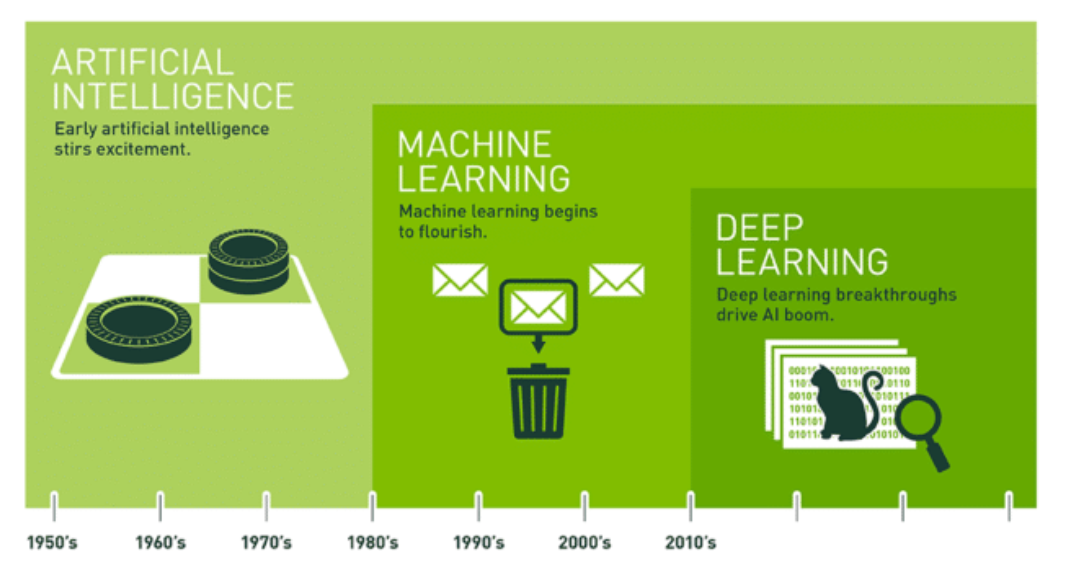
\includegraphics[width=0.5\linewidth]{bachelor_images/nvidia_ai_hierarchy.png}
    \caption{The hierarchy of artificial intelligence, machine learning and deep learning \cite{francuz}}
    \label{fig:hierarchy-ai-ml-dl}
\end{figure}

\subsection{Artificial Intelligence}
Artificial intelligence can be succinctly described as "the effort to automate intellectual tasks normally performed by humans." The field of AI encompasses various approaches, including machine learning and deep learning, which rely on data and statistical models to identify patterns and make decisions. However, the field also includes symbolic AI, which operates differently by relying solely on predefined rules rather than data-driven models \cite{francuz}. An example of symbolic AI is expert systems like MYCIN, which used around 500 of IF-THEN rules to diagnose bacterial infections and recommend treatments with accuracy on par with human specialists and better than general practitioners \cite{mycin}.

\subsection{Machine Learning}
On the other hand, machine learning is a branch of artificial intelligence in which the machine is trained rather than explicitly programmed, by making inferences from the input data it is presented with \cite{francuz}. Two major types of machine learning are supervised and unsupervised learning.

Supervised learning refers to an approach that relies on labeled datasets to train or "supervise" the model. The model is provided with input data along with the correct output, allowing it to learn by example. The model analyzes the relationship between the input features and the corresponding labels, gradually improving its ability to make accurate predictions. Supervised learning is commonly used for tasks such as classification, where data is sorted into categories, and regression, where numerical values are predicted based on patterns in the data. This method is widely applied in real-world scenarios like email spam detection, image recognition, and sales forecasting.

In contrast, unsupervised learning involves the model analyzing, clustering unlabeled data and identifying patterns without guidance from the programmer or datasets, hence it is called unsupervised learning. Unsupervised learning can be used to identify groups of products often purchased together \cite{supervised_ibm}.

In this project, we primarily employ supervised learning to develop our solution. This choice is driven by the nature of the problem, which involves identifying coupons from a screen view presented as an XML tree and extracting relevant data from them. Since this task is essentially a classification problem — where the goal is to categorize elements rather than uncover hidden patterns or group data points — supervised learning is the most suitable approach. By leveraging labeled data, the model can effectively learn to recognize and extract the desired information with accuracy and efficiency.

\subsection{Deep Learning}
Deep learning is a subset of machine learning wherein multilayered neural networks, called deep neural networks, are utilized to learn increasingly meaningful representations with each successive layer as seen in ~\ref{fig:nn_simple}; each representation is increasingly different from the original and more useful to determining the result. Traditionally, machine learning models focus on learning one or two layers of representations of the data \cite{francuz}, deep learning employs at least three layers, and typically hundreds or thousands of layers to train the models \cite{ibm_dl}.

\begin{figure}
    \centering
    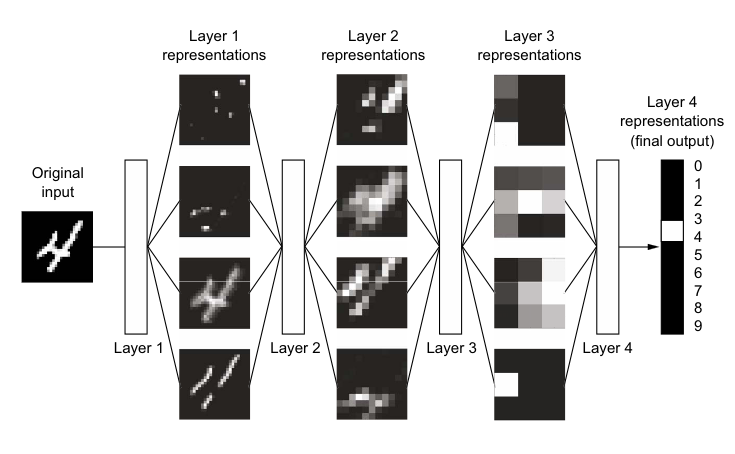
\includegraphics[width=0.5\linewidth]{bachelor_images/nn_simple.png}
    \caption{Data representations learned by a digit-classification model \cite{francuz}}
    \label{fig:nn_simple}
\end{figure}

The transformation implemented by a layer is defined (parametrized) by its \textit{weights}, which are numerical parameters. Learning involves adjusting these weights to ensure the network accurately maps inputs to their corresponding targets. A deep neural network can have millions of parameters, making it challenging to find the right values since changing one parameter affects the others. To guide this process, a \textit{loss function} measures how far the network's predictions deviate from the expected results, providing a score that reflects its performance. Deep learning relies on using the loss score as feedback to adjust the network's weights, guided by the optimizer using the backpropagation algorithm. Initially, the weights are random, resulting in poor predictions and a high loss score. With each example, the optimizer tweaks the weights to reduce the loss. Repeating this process across many examples gradually minimizes the loss, producing a trained network that closely matches its target outputs. This process is exemplified in ~\ref{fig:nn_function} \cite{francuz}.

\begin{figure}
    \centering
    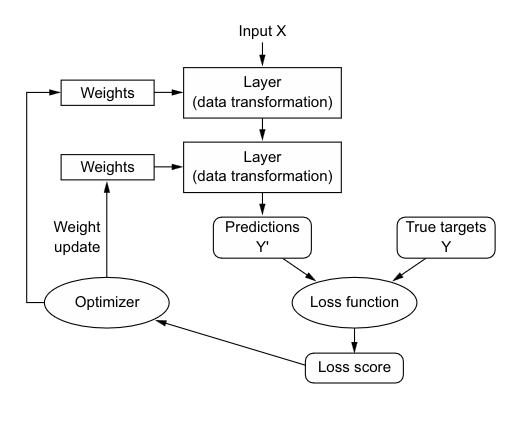
\includegraphics[width=0.5\linewidth]{bachelor_images/nn_function.png}
    \caption{A visualization of how a Deep Learning model works \cite{francuz}}
    \label{fig:nn_function}
\end{figure}

The advancement of deep learning contributed to the development of generative AI such as ChatGPT as well as Natural Language Processing (NLP) which enables machines understand and generate text and speech. This is useful for translations and extracting meaning from large quantities of data \cite{ibm_dl}.

% \subsection{Assessing the model - benchmarking}
% Benchmarking is the process of running a set of, among others, computer programs against a set of tests to assess their relative performance or precision \cite{benchmark}. Benchmarks are employed to evaluate and quantify the efficiency, accuracy, speed, and other metrics of a machine learning model or pipeline, thereby enabling the selection of the best overall solution to our problem.


\subsection{Transformers}
Transformers are deep learning models introduced in the 2017 paper "Attention Is All You Need" by Vaswani et al., which have significantly impacted natural language processing and other sequential data tasks. Unlike traditional recurrent neural networks (RNNs), transformers utilize self-attention mechanisms to process input data in parallel, enhancing efficiency and scalability. This architecture has become foundational in models like BERT, and GPT \cite{medium_t}.
\subsubsection{Model architecture}
The proposed architecture has a encoder-decoder structure wherein, given a sequence of input symbols $ (x_1, ... , x_n) $, the encoder computes a sequence of continuous vector representations $ z = (z_1, ... , z_n) $, where each encodes contextual information about the corresponding within the entire input sequence. The decoder takes $ z $ and outputs a sequence $ (y_1, ... , y_n) $. At every step, the model utilizes previously-generated symbols as additional input when creating the next output. This is shown in figure ~\ref{fig:transformers_fig}.

The encoder consists of multiple layers, each typically comprising of two parts: a multi-head self-attention mechanism and a simple fully connected feed-forward network. Residual connection and layer normalization is utilized to improve model performance.

Similarly, the decoder has a similar structure. In addition to the two parts in the encoder, each layer performs attention over the encoder’s output. To ensure the model does not look ahead in the sequence, the self-attention in the decoder is modified to prevent the model from attending to future positions, so each prediction only depends on earlier information.

\begin{figure}
    \centering
    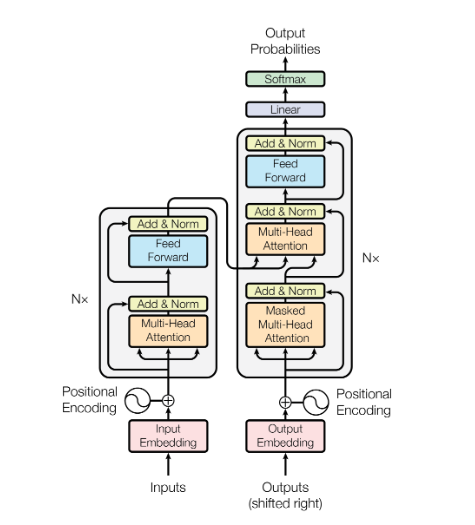
\includegraphics[width=0.5\linewidth]{bachelor_images/transformer_arch.png}
    \caption{Transformer Architecture \cite{attention}}
    \label{fig:transformers_fig}
\end{figure}

\subsubsection{Attention and multi-head attention}
The attention mechanism is the core innovation of transformers. It allows the model to weigh the importance of each word (or token) in a sequence with respect to every other word. This is done by computing a set of attention scores, which decide how much attention one word should pay to others in the sequence.
Multi-head attention is a key component of transformer architectures, enabling models to focus on different parts of an input sequence simultaneously. It works by projecting the input data into multiple subspaces, each corresponding to a separate attention head. These heads independently process the data, capturing various relationships and features. The outputs are then concatenated and transformed to produce the final result \cite{attention}.
This approach allows the model to attend to multiple aspects of the input, such as different positions or semantic relationships, enhancing its ability to understand complex patterns. For example, in natural language processing tasks, one attention head might focus on syntactic structures while another captures semantic nuances.
By distributing the attention mechanism across multiple heads, transformers can efficiently process information in parallel, leading to improved performance in tasks like machine translation, text summarization, and language understanding \cite{medium_medium_t}.
The relationship between attention and multi-head attention is depicted in figure ~\ref{fig:attention_fig}.

\begin{figure}
    \centering
    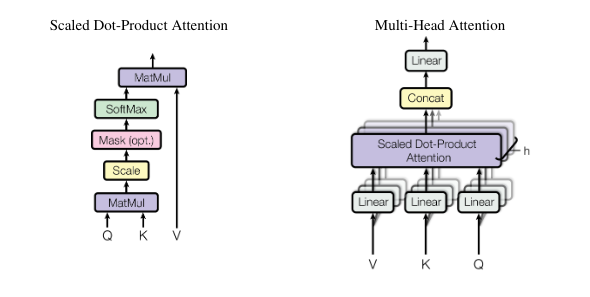
\includegraphics[width=0.7\linewidth]{bachelor_images/attention_fig.png}
    \caption{Attention and multi-head attention \cite{attention}}
    \label{fig:attention_fig}
\end{figure}


\subsection{Quantization}
Quantization is a technique employed in many fields including machine learning, to reduce the precision of numerical representations within models, typically converting high-precision formats like 32-bit floating point (FP32) to lower-precision formats such as 8-bit integers (INT8). Using integer operations instead of floating-point reduces the computational and memory requirements during inference, thereby making it more efficient and faster, which is an essential benefit for real-time applications. Furthermore, quantization enables deployment on resource-constrained hardware such as smartphones and tablets, while also reducing power consumption due to lighter computational loads. Though this may slightly reduce model accuracy, the trade-off often proves worthwhile in practical applications \cite{ibm_quantization}.
The two most common quantization techniques are float32 -> float16 and float32 -> int8 \cite{quant_hf}.
\subsubsection{float32 -> float16}
Performing quantization from float32 to float16 is relatively straightforward as both data types are represented in the same manner. Float32 has the following format:
\begin{enumerate}
	\item The most significant bit (MBS) represents the sign of the number, ie. whether it is negative or positive.
	\item The next 8 bits represent the exponent.
	\item The remaining 23 bits, are the mantissa, ie. the decimal.
\end{enumerate}

When converting from fromt32 to float16, we just remove the last 13 bits of the mantissa, creating a rounding error, and “shrinks” the exponent to fit into 5 bits. This may create a float overflow error if the float32 number is greater than $ 6.55e^4$ \cite{quant_explained}.


\subsubsection{float32 -> int8}
This type of quantization is more complicated as an int8 can only represent 256 values which is significantly less compared to the $ 2^24 $  values represented by a float32. The idea of this quantization is to find the best way to map float32 values into the int8 space, using the affine quantization scheme: $ x = S * (x_q - Z) $.
\begin{enumerate}
	\item $ x $ is the float32 value to be quantized.
	\item  $ x_q $ is the quantized int8 value associated with $ x $. It can be computed as follows $ x_q = round(x/S + Z) $.
	\item $ S \in float32$ is the scale.
	\item $ Z $ is the zero-point, which is the int8 value that corresponds to 0 in the float32 range \cite{quant_hf}.
\end{enumerate}


\subsection{Finetuning}
Fine-tuning is a specialized form of transfer learning that involves adapting a pre-trained model to perform a specific task, such as identifying coupons or extracting relevant information from them, rather than identifying all kinds of objects. Instead of training a model from scratch, fine-tuning starts with a model already trained on a large dataset and further trains it using a smaller, task-specific dataset. Attempting to train a large model from scratch on a small dataset can lead to overfitting, where the model performs well on training data but generalizes poorly to unseen data. This approach is particularly beneficial for deep learning models, such as large language models (LLMs) in natural language processing or convolutional neural networks (CNNs) in computer vision, as it reduces the computational resources and labeled data required \cite{ibm_finetuning}.
Fine-tuning consists of the following steps:
\begin{enumerate}
	\item Training a source model on a large, general-purpose dataset. This enables the model to learn broadly useful feature representations.
	\item Construct a new target model by copying the architecture and parameters of the source model, excluding its final output layer. The retained parameters are presumed to encode transferable knowledge, while the output layer—being specific to the source dataset —is discarded.
	\item Introduce a new output layer tailored to the target task, ensuring it matches the number of classes in the target dataset. Initialize this layer’s parameters randomly.
	\item Train the target model on the new, task-specific dataset (e.g., a dataset of coupons. The new output layer is trained from scratch, while the remaining layers are fine-tuned using the pre-trained weights as a starting point \cite{finetune_cool_image}.
\end{enumerate}

\section{Should We Be Afraid of AI? - Assessing the Risks and Ethical Implications of Artificial Intelligence}

As artificial intelligence becomes increasingly complex and integrated into our daily lives, the voices raising concerns about its dangers grow louder. Some express concern about the risks of excessive surveillance and privacy erosion, envisioning a future where AI systems are deeply intertwined with our surroundings, essentially hearing what we hear and seeing what we see \cite{sroka_vid}. Others highlight the environmental challenges tied to large-scale AI deployment, such as rising energy and water consumption, along with the need for rare materials in microchip production \cite{ai_env_concerns}. This section will focus on assessing the risks of artificial intelligence and how our solution will take them into account.

\subsection{Privacy Erosion}
AI systems heavily rely on vast amounts of user data to deploy machine learning techniques that identify subtle patterns and behaviors that may not be immediately evident, thus enabling personalized recommendations \cite{data_guard}. Social media platforms like TikTok exemplify this, as their algorithms suggest content based on users' previous interactions \cite{it_convergence} \cite{builtin}. While this personalization enhances user engagement, it also risks influencing people's opinions and shaping their worldview by trapping them in ideological echo chambers\cite{echo_chambers}.

Consequently, ‘information privacy’ is one of the primary concerns surrounding the use of AI. ‘Information privacy’ refers to the protection of personal data that is being collected, processed and stored by AI systems \cite{transcend}. Training machine learning models typically requires immense datasets, involving terabytes or even petabytes of information. Therefore, these training sets likely include sensitive user information such as healthcare records and biometric data \cite{ibm_vast_data}. Beyond explicit data collection, AI systems can also infer highly personal attributes, such as political beliefs, sexual orientation, or health conditions, from seemingly unrelated data — a phenomenon known as 'predictive harm' \cite{transcend}. This information can be utilized to subject individuals to targeted advertising, unwanted profiling, and even identity theft, often without the user’s consent or awareness \cite{data_guard}, thus posing a serious privacy risk.

Moreover, AI systems can pose ‘autonomy harms’, wherein the insights derived from data are used to influence individuals' decisions or behavior without their knowledge or proper consent. The common mindset of having "nothing to hide" overlooks the broader implications of these practices, which can undermine personal freedom and informed decision-making. A significant example of this problem is the Facebook-Cambridge Analytica scandal, in which a seemingly benign personality quiz was utilized to harvest over 87 million Facebook users’ data. Based on this data, detailed psychological profiles were constructed and leveraged to target individuals with personalized political ads during the 2016 US Presidential Election. This case underscores how AI can extract deeply personal insights from mundane user interactions, demonstrating the potential for misuse when data privacy protections are inadequate \cite{transcend}.

To address privacy concerns associated with AI systems, we are implementing locally-deployable models that process data directly on users' devices. This ensures that raw, unprocessed information never leaves the device or gets transmitted to external servers. By keeping data local, we significantly reduce the risk of unauthorized access, data breaches, or misuse. This approach empowers users with greater control over their information while still benefiting from the capabilities of AI in a secure and privacy-conscious manner.

\subsection{Environmental Concerns}
AI has a notable carbon footprint due to its increasing energy consumption, particularly during model training and usage \cite{forbes_dl_env}. One study predicts that by 2027, AI-related energy consumption could reach 85–134 TWh \cite{this_study}, representing nearly 0.5\% of today's global electricity usage. This estimate is based on the energy consumption of the Nvidia A100 servers - the hardware estimated to be used by 95 percent of the A.I. market, and their projected sales in the upcoming years \cite{nyt_el}. Training LLMs typically requires significantly more energy in comparison to making a single prediction on the trained model \cite{sci_dir_comp}, for instance BERT required "the energy of a round-trip transcontinental flight" to train, while GPT-3 emitted 552 metric tons of carbon dioxide which is "the equivalent of 123 gasoline-powered passenger vehicles driven for one year" \cite{sci_am_co2}.

Furthermore, while a quarter of the world lacks access to clean water and sanitation, data centers consume significant quantities of water during their construction and during operation to cool electrical components \cite{first}. AI server cooling requires up to 9 liters of water per kWh of energy used. Given the amount of energy required to train and operate a model, this will exacerbate the lack of water, with UN estimates stating that by 2030 half of the world’s population will be facing severe water stress \cite{water_scarcity}. It is estimated that globally, infrastructure related to AI will soon require six times more water than Denmark \cite{first}.

In our approach, we opted to fine-tune existing language models rather than train new ones from scratch, a decision driven by both computational efficiency and environmental considerations. As highlighted by Wang et al. (2023), pre-training a model like BERT can require the equivalent energy of anywhere from 400 to 45,000 fine-tuning runs, depending on the dataset size. Their analysis shows that the number of training tokens is a reliable heuristic for estimating energy use during fine-tuning, and that sequence length significantly impacts energy intensity during this phase. These findings emphasize the substantial energy and carbon costs associated with pre-training, underscoring the environmental benefits of leveraging pre-trained models for downstream tasks \cite{finetuning_env_good}.

\chapter{Overview of Existing Solutions}

To the best of our knowledge, at the time of this project's commissioning, no publicly available solutions directly addressed this problem. The most comparable approaches involve existing multimodal models. While widely used models such as ChatGPT and Gemini provide general data extraction capabilities~\cite{brinkmann2023}, they are unsuitable for our task due to their substantial computational requirements. A key limitation of these models is their large size—for example, GPT-3 consists of 175 billion parameters\cite{chatgpt_params}—rendering them impractical for deployment on mobile devices~\cite{LinguaLinked}.

Alternatively, computer vision models can be used to extract text and bounding boxes from screen images. Microsoft’s OmniParser~\cite{omniparser_intro}, for instance, has demonstrated strong performance on the ScreenSpot dataset~\cite{omniparser_intro, cheng2024}. However, the challenge of organizing extracted text into structured coupon data renders this approach unsuitable for our study. Furthermore, our experiments with running OmniParser locally on example images indicate that it relies on CUDA technology, making it impractical for deployment on mobile devices.

\section{Murmuras' existing solution}
Murmuras' current approach relies on a set of fixed scrapping programms tailored to specific layouts from limited set of applications, making it inflexible and expansive to generalize across diverse coupon formats. This lack of adaptability limits its usefulness in real-world scenarios where coupon structures vary widely. Since our goal is to develop a solution that is easily adaptable for processing diverse mobile content, this method is not well-suited for our needs.

In contrast, Murmuras' most-recent proof of concept involves wrapping the \texttt{CSV} data with a prompt that instructs the model and sending it to GPT-4o-mini. This approach leverages an LLM to interpret the data to extract relevant coupon details. However, the reliance on an external server means the solution does not run locally on the mobile device, leading to potential privacy concerns, latency issues, and a dependence on internet connectivity.

\section{Scapegraph AI}
ScrapeGraphAI is an open-source library that streamlines data extraction from websites and local documents by utilizing LLMs and graph logic to construct scraping pipelines \cite{scapegraph_repo}. The library supports integration with various LLMs, including local models through the use of Ollama \cite{ollama_repo} \cite{scapegraph_usage}.

However, Scrapepraph AI provides only Python and Node.js SDKs \cite{scapegraph_sdks}, which could prove to be an issue with regard to mobile deployment, because neither Python nor Node.js is natively supported on iOS or Android \cite{android_dev_site} \cite{ios_dev_site}.

Moreover, due to mobile devices typically having limited processing power and memory compared to desktop computers or servers \cite{mobile_resources}, we cannot solely rely on the size of the model in order to improve performance. We believe that through fine-tuning LLMs, we are able to develop tools that are far more viable for edge device usage.

\chapter{Technologies}

\section{General}

The main platforms used during the development process were Hugging Face\cite{hugging-face} and GitHub\cite{github}. Hugging Face served as a hub for storing and managing both trained machine learning models and datasets. During development, we also made extensive use of several Python libraries provided by Hugging Face, including \textit{datasets}\cite{lhoest2021datasetscommunitylibrarynatural}, \textit{transformers}\cite{wolf-etal-2020-transformers}, and \textit{evaluate}\cite{evaluate}. GitHub, in turn, offered version control for our code and documentation, and supported DevOps tasks such as issue tracking and automated unit testing.

Python\cite{python} was the primary programming language used, due to its broad support for machine learning workflows. Additionally, some auxiliary experiments related to Android deployment were conducted using Kotlin\cite{kotlin}\cite{service_demo_app_repo}.

\section{LLaMA Proposal}

Our first solution was based on the LLaMA architecture and utilized a custom fine-tuned version of LLaMA-3.2-1b provided by Meta\cite{meta-llama}. Fine-tuning was performed using the Unsloth\cite{unsloth} tool, which enabled efficient resource usage. Specifically, Unsloth applied the LoRA (Low-Rank Adaptation) fine-tuning technique\cite{hu2021loralowrankadaptationlarge}, reducing the number of trainable parameters to approximately 10 million. It also facilitated easy model conversion to the GGUF format.

The fine-tuning process was carried out on the Modal platform\cite{modal}, which allowed us to define execution environments directly in Python and execute code on cloud infrastructure equipped with H100 GPUs. Training progress and logs were monitored using Weights \& Biases (Wandb)\cite{wandb}.

Model inference was conducted using the Llama.cpp\cite{llama-cpp} tool, utilizing the model converted to the GGUF format.

\section{BERT Proposal}

The second approach—a two-stage BERT pipeline—was also trained on the Modal platform. Logging and experiment tracking were similarly managed using Wandb.

\section{Auxiliary Experiments}

Additional experiments conducted as part of this project involved frameworks such as SpaCy\cite{spacy}\cite{spacy-exp} and Scrapegraph AI\cite{scapegraph_repo}\cite{scrapegraph-exp}, as well as mobile deployment tools including ONNX\cite{onnx}\cite{onnx-exp}, liteRT\cite{lite-rt}\cite{lite-rt-exp}, and Executorch\cite{executorch}\cite{executorch-exp}. These experiments were developed using Android Studio\cite{android-studio}\cite{service_demo_app_repo} and Jupyter notebooks\cite{jupyter}, running in an IPython\cite{ipython} environment.


% \section{}

% \chapter{Technologies}
% \chapter{Architecture design}
% \chapter{Pipelines}
% \chapter{Benchmark}
% \chapter{Performance}
% \chapter{Possible extensions}
% \chapter{Conclusion}
% \chapter{Charts}

\begin{thebibliography}{99}

\addcontentsline{toc}{chapter}{Bibliography}
\raggedright

\bibitem{murmuras}
\textit{Murmuras website}.
\url{https://murmuras.com/}.
[Accessed 2025-02-11].

\bibitem{seo2023}
\textit{Seo, D., \& Yoo, Y. (2023). Improving Shopping Mall Revenue by Real-Time Customized Digital Coupon Issuance. IEEE Access, 11, 7924–7932.}
\url{https://doi.org/10.1109/ACCESS.2023.3239425}

\bibitem{coupon_definition}
\textit{Britannica Dictionary definition of COUPON}.
\url{https://www.britannica.com/dictionary/coupon}.
[Accessed 2025-02-03].

\bibitem{nayal2021}
\textit{Nayal, P., \& Pandey, N. (2021). What Makes a Consumer Redeem Digital Coupons? Behavioral Insights from Grounded Theory Approach. *Journal of Promotion Management*, 28(3), 205–238.}
\url{https://doi.org/10.1080/10496491.2021.1989541}

\bibitem{danaher2015}
\textit{Danaher, P. J., Smith, M. S., Ranasinghe, K., \& Danaher, T. S. (2015). *Where, when, and how long: Factors that influence the redemption of mobile phone coupons.* *Journal of Marketing Research*, *52*(5), 710--725.}
\url{https://journals.sagepub.com/doi/full/10.1509/jmr.13.0341}

\bibitem{jayadharshini2023}
\textit{Jayadharshini, P., Sharon Roji, Priya. C, Lalitha, K., Santhiya, S., Keerthika, S., \& Abinaya, N. (2023). *Enhancing Retailer Auctions and Analyzing the Impact of Coupon Offers on Customer Engagement and Sales Through Machine Learning.* *2023 Intelligent Computing and Control for Engineering and Business Systems (ICCEBS)*, 1–6. }
\url{https://doi.org/10.1109/ICCEBS58601.2023.10448900}

\bibitem{design_of_coupons}
Xiong Keyi, Yang Wensheng
\textit{Research on the Design of E-coupons for Directional Marketing of Two Businesses in Competitive Environment}.
\url{https://www.sciencepublishinggroup.com/article/10.11648/j.ijefm.20200801.16}.
[Accessed 2025-02-04].

\bibitem{li2024}
\textit{Li, J. (2024). The evolution, applications, and future prospects of large language models: An in-depth overview. Applied and Computational Engineering 35, 234–244.}\url{https://doi.org/10.54254/2755-2721/35/20230399}

\bibitem{sui2024}
\textit{Sui, Y., Zhou, M., Zhou, M., Han, S., \& Zhang, D. (2024). Table meets LLM: Can large language models understand structured table data? A benchmark and empirical study. Proceedings of the 17th ACM International Conference on Web Search and Data Mining, 645--654.}

\bibitem{targeted_reminders}
Li Li, et. al.
\textit{Targeted reminders of electronic coupons: using predictive analytics to facilitate coupon marketing}.
\url{https://link.springer.com/article/10.1007/s10660-020-09405-4}.
[Accessed 2025-02-04].

\bibitem{competitor_tariffs}
Bernhard König, et. al.
\textit{Analysing competitor tariffs with machine learning}.
\url{https://www.milliman.com/en/insight/analysing-competitor-tariffs-with-machine-learning}.
[Accessed 2025-02-04].

\bibitem{ml_general}
Iqbal H. Sarker
\textit{Machine Learning: Algorithms, Real-World Applications and Research Directions}.
\url{https://link.springer.com/article/10.1007/s42979-021-00592-x}.
[Accessed 2025-02-05].

\bibitem{emarketer_coupon_stats}
Sara Lebow
\textit{How consumers access digital coupons}.
\url{https://www.emarketer.com/content/how-consumers-access-digital-coupons}.
[Accessed 2025-02-05].

\bibitem{coupon_stats_2}
\textit{Unveiling IT Coupons Trends and Statistics}
\url{https://www.go-globe.com/unveiling-it-coupons-trends-statistics/}.
[Accessed 2025-02-05].

\bibitem{android_view}
\textit{Android API Reference - View}
\url{https://developer.android.com/reference/android/view/View}
[Accessed 2025-03-11]

\bibitem{brinkmann2023}
\textit{Brinkmann, A., Shraga, R., Der, R. C., \& Bizer, C. (2023). Product Information Extraction using ChatGPT. arXiv preprint, arXiv:2306.14921.}
\url{https://arxiv.org/abs/2306.14921}

\bibitem{chatgpt_params}
\textit{Tom B. Brown, Benjamin Mann, Nick Ryder, Melanie Subbiah, Jared
Kaplan, Prafulla Dhariwal, Arvind Neelakantan, Pranav Shyam, Girish
Sastry, Amanda Askell, Sandhini Agarwal, Ariel Herbert-Voss, Gretchen
Krueger, Tom Henighan, Rewon Child, Aditya Ramesh, Daniel M.
Ziegler, Jeffrey Wu, Clemens Winter, Christopher Hesse, Mark Chen,
Eric Sigler, Mateusz Litwin, Scott Gray, Benjamin Chess, Jack Clark,
Christopher Berner, Sam McCandlish, Alec Radford, Ilya Sutskever, and
Dario Amodei. Language models are few-shot learners, 2020}

\bibitem{scapegraph_repo}
Marco Perini, Lorenzo Padoan, Marco Vinciguerra
\textit{Scrapegraph-ai}.
\url{https://github.com/VinciGit00/Scrapegraph-ai}.
[Accessed 2025-02-24].

\bibitem{ollama_repo}
\textit{Ollama}.
\url{https://github.com/ollama/ollama}.
[Accessed 2025-02-24].

\bibitem{scapegraph_usage}
Marco Perini, Lorenzo Padoan, Marco Vinciguerra
\textit{Scrapegraph-ai usage}.
\url{https://github.com/ScrapeGraphAI/Scrapegraph-ai?tab=readme-ov-file#-usage}.
[Accessed 2025-02-24].

\bibitem{scapegraph_sdks}
Marco Perini, Lorenzo Padoan, Marco Vinciguerra
\textit{Scrapegraph-ai API and SDKs}.
\url{https://github.com/ScrapeGraphAI/Scrapegraph-ai?tab=readme-ov-file#-scrapegraph-api--sdks}.
[Accessed 2025-02-24].

\bibitem{android_dev_site}
\textit{Android developer fundamentals website}.
\url{https://developer.android.com/guide/components/fundamentals}.
[Accessed 2025-02-24].

\bibitem{ios_dev_site}
\textit{Apple developer website}.
\url{https://developer.apple.com/develop/}.
[Accessed 2025-02-24].

\bibitem{omniparser_intro}
\textit{Yadong Lu, Jianwei Yang, Yelong Shen, and Ahmed Awadallah. Omni-
parser for pure vision based gui agent, 2024.}

\bibitem{cheng2024}
\textit{Cheng, K., Sun, Q., Chu, Y., Xu, F., Li, Y., Zhang, J., \& Wu, Z. (2024). SeeClick: Harnessing GUI Grounding for Advanced Visual GUI Agents. arXiv preprint, arXiv:2401.10935.} \url{https://arxiv.org/abs/2401.10935}

\bibitem{mobile_resources}
Xiang Li, et. al.
\textit{Large Language Models on Mobile Devices: Measurements, Analysis, and Insights}
\url{https://dl.acm.org/doi/10.1145/3662006.366205}

\bibitem{LinguaLinked}
Junchen Zhao, et. al.
\textit{LinguaLinked: A Distributed Large Language Model Inference System for Mobile Devices}
\url{https://arxiv.org/pdf/2312.00388}

\bibitem{sequence_matcher}
\textit{difflib — Helpers for computing deltas}
\url{https://docs.python.org/3/library/difflib.html}

\bibitem{francuz_1}
page 1
\textit{Deep Learning with Python}
\url{https://sourestdeeds.github.io/pdf/Deep%20Learning%20with%20Python.pdf}

\bibitem{francuz_2}
pages 2 and 3
\textit{Deep Learning with Python}
\url{https://sourestdeeds.github.io/pdf/Deep%20Learning%20with%20Python.pdf}

\bibitem{francuz_3}
pages 3 and 4
\textit{Deep Learning with Python}
\url{https://sourestdeeds.github.io/pdf/Deep%20Learning%20with%20Python.pdf}

\bibitem{francuz_8}
pages 7 and 8
\textit{Deep Learning with Python}
\url{https://sourestdeeds.github.io/pdf/Deep%20Learning%20with%20Python.pdf}

\bibitem{francuz_9}
pages 8 - 10
\textit{Deep Learning with Python}
\url{https://sourestdeeds.github.io/pdf/Deep%20Learning%20with%20Python.pdf}

\bibitem{nvidiaimage}
\textit{What’s the Difference Between Artificial Intelligence, Machine Learning and Deep Learning?}
\url{https://blogs.nvidia.com/blog/whats-difference-artificial-intelligence-machine-learning-deep-learning-ai/}

\bibitem{ibm_ai}
\textit{What is artificial intelligence (AI)?}
\url{https://www.ibm.com/think/topics/artificial-intelligence}

\bibitem{ibm_privacy}
\textit{Exploring privacy issues in the age of AI}
\url{https://www.ibm.com/think/insights/ai-privacy}

\bibitem{mycin}
\textit{MYCIN}
\url{https://www.britannica.com/technology/MYCIN}

\bibitem{supervised_ibm}
\textit{Supervised versus unsupervised learning: What's the difference?}
\url{https://www.ibm.com/think/topics/supervised-vs-unsupervised-learning}

\bibitem{benchmark}
\textit{Computer Benchmark}.
\url{https://bhatabhishek-ylp.medium.com/benchmarking-in-computer-c6d364681512}.
[Accessed 2025-02-03].

\bibitem{not_sroka_vid}
\textit{The privacy paradox with AI}.
\url{https://www.reuters.com/legal/legalindustry/privacy-paradox-with-ai-2023-10-31/}.
[Accessed 2025-03-24].

\bibitem{ai_scare2}
\textit{Beware the Privacy Violations in Artificial Intelligence Applications}
\url{https://www.isaca.org/resources/news-and-trends/isaca-now-blog/2021/beware-the-privacy-violations-in-artificial-intelligence-applications}
[Accessed 2025-04-01]

\bibitem{ai_scare3}
\textit{AI – the threats it poses to reputation, privacy and cyber security, and some practical solutions to combating those threats}
\url{https://www.taylorwessing.com/en/global-data-hub/2024/cyber-security---weathering-the-cyber-storms/ai---the-threats-it-poses-to-reputation}

\bibitem{ai_env_concerns}
\textit{AI has an environmental problem. Here’s what the world can do about that.}
\url{https://www.unep.org/news-and-stories/story/ai-has-environmental-problem-heres-what-world-can-do-about}
[Accessed 2025-03-24]

\bibitem{it_convergence}
\textit{Top Use Cases of AI-Based Recommendation Systems}.
\url{https://www.itconvergence.com/blog/top-use-cases-of-ai-based-recommendation-systems/}.
[Accessed 2025-03-24].

\bibitem{builtin}
\textit{ 14 Risks and Dangers of Artificial Intelligence (AI)}.
\url{https://builtin.com/artificial-intelligence/risks-of-artificial-intelligence}.
[Accessed 2025-03-24].

\bibitem{data_guard}
\textit{The growing data privacy concerns with AI: What you need to know}.
\url{https://www.dataguard.com/blog/growing-data-privacy-concerns-ai/}.
[Accessed 2025-03-24].

\bibitem{transcend}
\textit{Examining Privacy Risks in AI Systems}.
\url{https://transcend.io/blog/ai-and-privacy}.
[Accessed 2025-03-24].

\bibitem{ibm_vast_data}
\textit{Exploring privacy issues in the age of AI}.
\url{https://www.ibm.com/think/insights/ai-privacy}.
[Accessed 2025-03-24].


\bibitem{forbes_dl_env}
\textit{Deep Learning’s Carbon Emissions Problem}.
\url{https://www.forbes.com/sites/robtoews/2020/06/17/deep-learnings-climate-change-problem/}.
[Accessed 2025-03-24].

\bibitem{this_study}
\textit{The growing energy footprint of artificial intelligence}.
\url{https://www.researchgate.net/publication/374598219_The_growing_energy_footprint_of_artificial_intelligence}.
%https://www.cell.com/joule/pdf/S2542-4351(23)00365-3.pdf
[Accessed 2025-04-16].

\bibitem{nyt_el}
\textit{A.I. Could Soon Need as Much Electricity as an Entire Country}.
\url{https://www.nytimes.com/2023/10/10/climate/ai-could-soon-need-as-much-electricity-as-an-entire-country.html}.
[Accessed 2025-03-24].

\bibitem{sci_dir_comp}
\textit{Trends in AI inference energy consumption: Beyond the performance-vs-parameter laws of deep learning}.
\url{https://www.sciencedirect.com/science/article/pii/S2210537923000124#sec7}.
[Accessed 2025-03-24].

\bibitem{sci_am_co2}
\textit{A Computer Scientist Breaks Down Generative AI’s Hefty Carbon Footprint}.
\url{https://www.scientificamerican.com/article/a-computer-scientist-breaks-down-generative-ais-hefty-carbon-footprint/}.
[Accessed 2025-03-24].

\bibitem{water_scarcity}
\textit{AI Is Accelerating the Loss of Our Scarcest Natural Resource: Water}.
\url{https://www.forbes.com/sites/cindygordon/2024/02/25/ai-is-accelerating-the-loss-of-our-scarcest-natural-resource-water/}.
[Accessed 2025-03-24].

\bibitem{first}
\textit{AI has an environmental problem. Here’s what the world can do about that.}.
\url{https://www.unep.org/news-and-stories/story/ai-has-environmental-problem-heres-what-world-can-do-about}.
[Accessed 2025-03-24].

\bibitem{ibm_dl}
\textit{What is deep learning?}.
\url{https://www.ibm.com/think/topics/deep-learning}.
[Accessed 2025-03-24].

\bibitem{BERT_intro}
\textit{BERT: Pre-training of Deep Bidirectional Transformers for Language Understanding}.
\url{https://arxiv.org/abs/1810.04805v2}.
[Accessed 2025-04-04]

\bibitem{BERT_hf}
\textit{BERT model page on hf}.
\url{https://huggingface.co/google-bert/bert-base-uncased}.
[Accessed 2025-04-04]

\bibitem{Region_proposal}
\textit{Faster R-CNN: Towards Real-Time Object Detection with Region Proposal Networks}
\url{https://arxiv.org/abs/1506.01497}
[Accessed 2025-04-04]

\bibitem{RoBERTa}
\textit{RoBERTa: A Robustly Optimized BERT Pretraining Approach}.
\url{https://arxiv.org/abs/1907.11692}
[Accessed 2025-04-04]

\bibitem{ALBERT}
\textit{ALBERT: A Lite BERT for Self-supervised Learning of Language Representations}.
\url{https://arxiv.org/abs/1909.11942}
[Accessed 2025-04-04]

\bibitem{ALBERT_hf}
\textit{ALBERT model page on hf}.
\url{https://huggingface.co/albert/albert-base-v2}.
[Accessed 2025-04-04]

\bibitem{DISTILBERT}
\textit{DistilBERT, a distilled version of BERT: smaller, faster, cheaper and lighter}
\url{https://arxiv.org/abs/1910.01108}
[Accessed 2025-04-04]

\bibitem{BERT_comp}
\textit{Comparative Analysis of BERT Variants for Text Detection Tasks}
\url{https://www.researchgate.net/publication/385142549_Comparative_Analysis_of_BERT_Variants_for_Text_Detection_Tasks}
[Accessed 2025-04-04]

\bibitem{FBAIHF}
\textit{Facebook AI on HuggingFace}
\url{https://huggingface.co/FacebookAI}
[Accessed 2025-04-04]

\bibitem{BERT_multiling}
\textit{Multilingual BERT on HuggingFace}
\url{https://huggingface.co/google-bert/bert-base-multilingual-cased}
[Accessed 2025-04-04]

\bibitem{ModernBERTPaper}
\textit{Smarter, Better, Faster, Longer: A Modern Bidirectional Encoder for Fast, Memory Efficient, and Long Context Finetuning and Inference}
\url{https://arxiv.org/abs/2412.13663}
[Accessed 2025-04-05]

\bibitem{ModernBERThf}
\textit{ModernBERT on HiggingFace}
\url{https://huggingface.co/answerdotai/ModernBERT-base}
[Accessed 2025-04-05]

\bibitem{CurrLearn}
\textit{Curriculum learning}
\url{https://dl.acm.org/doi/abs/10.1145/1553374.1553380}
[Accessed 2025-04-07]

\bibitem{echo_chambers}
The echo chamber effect on social media
\url{https://pubmed.ncbi.nlm.nih.gov/33622786/}
[Accessed 2025-04-09]

\bibitem{finetuning_env_good}
Energy and Carbon Considerations of Fine-Tuning BERT
\url{https://arxiv.org/html/2311.10267}
[Accessed 2025-04-09]

\bibitem{ibm_finetuning}
What is fine-tuning?
\url{https://www.ibm.com/think/topics/fine-tuning}
[Accessed 2025-04-09]

\bibitem{finetune_cool_image}
14.2. Fine-Tuning
\url{https://d2l.ai/chapter_computer-vision/fine-tuning.html}
[Accessed 2025-04-09]

\bibitem{ibm_quantization}
What is quantization?
\url{https://www.ibm.com/think/topics/quantization/}
[Accessed 2025-04-09]

\bibitem{quant_hf}
Quantization
\url{https://huggingface.co/docs/optimum/en/concept_guides/quantization}
[Accessed 2025-04-09]

\bibitem{quant_explained}
Float32 vs Float16 vs BFloat16?
\url{https://newsletter.theaiedge.io/p/float32-vs-float16-vs-bfloat16}
[Accessed 2025-04-09]

\bibitem{attention}
Attention Is All You Need
\url{https://arxiv.org/pdf/1706.03762}
[Accessed 2025-04-08]

\bibitem{medium_medium_t}
Exploring Multi-Head Attention: Why More Heads Are Better Than One
\url{https://medium.com/%40hassaanidrees7/exploring-multi-head-attention-why-more-heads-are-better-than-one-006a5823372b}
[Accessed 2025-04-08]

\bibitem{medium_t}
Understanding the Transformer Model: A Report on “Attention Is All You Need” by Ashish Vaswani et al.
\url{https://medium.com/%40shivayapandey359/attention-is-all-you-need-26586e6ab8ca}
[Accessed 2025-04-08]

\bibitem{pp}
\textit{Pareto principle}
\url{https://en.wikipedia.org/wiki/Pareto_principle}
[Accessed 2025-04-10]

\bibitem{iob2}
\textit{Named Entity Recognition}
\url{https://cs229.stanford.edu/proj2005/KrishnanGanapathy-NamedEntityRecognition.pdf}
[Accessed 2025-04-10]

\bibitem{meta-llama}
\textit{Llama 3.2 published by Meta}
\url{https://ai.meta.com/blog/llama-3-2-connect-2024-vision-edge-mobile-devices/}
[Accessed 2025-04-17]

\bibitem{unsloth}
\textit{Unsloth}
\url{https://unsloth.ai/}
[Accessed 2025-04-17]

\bibitem{hugging-face}
\textit{The Hugging Face Platform}
\url{https://huggingface.co/}
[accessed 17.04.2025]

\bibitem{github}
\textit{The Github platform}
\url{https://github.com/}
[accessed 17.04.2025]

\bibitem{modal}
\textit{The Modal platform}
\url{https://modal.com/}
[accessed 17.04.2025]

\bibitem{wandb}
\textit{The Wandb platform}
\url{https://wandb.ai/}
[accessed 17.04.2025]

\bibitem{python}
\textit{The website of Python programming language}
\url{https://www.python.org/}
[accessed 17.04.2025]

\bibitem{service_demo_app_repo}
\textit{Our experiment with mobile app that runs in background}
\url{https://github.com/ZPP-MURMURAS/ZPP_Murmuras/tree/main/research/service_demo_app}

\bibitem{kotlin}
\textit{Webpage of the Kotlin programming Language}
\url{https://kotlinlang.org/}
[accessed 24.04.2025]

\bibitem{hu2021loralowrankadaptationlarge}
\textit{dward J. Hu and Yelong Shen and Phillip Wallis and Zeyuan Allen-Zhu and Yuanzhi Li and Shean Wang and Lu Wang and Weizhu Chen (2021): LoRA: Low-Rank Adaptation of Large Language Models}
\url{https://arxiv.org/abs/2106.09685}

\bibitem{triton}
\textit{Tillet, Philippe and Kung, H. T. and Cox, David (2019): Triton: an intermediate language and compiler for tiled neural network computations}
\url{https://doi.org/10.1145/3315508.3329973}

\bibitem{lhoest2021datasetscommunitylibrarynatural}
\textit{Lhoest et al (2021): Datasets: A Community Library for Natural Language Processing}
\url{https://arxiv.org/abs/2109.02846}

\bibitem{evaluate}
\textit{evaluate Python library}
\url{https://pypi.org/project/evaluate/}
[accessed 24.05.2025]

\bibitem{wolf-etal-2020-transformers}
\textit{Wolf et al (2020): Transformers: State-of-the-Art Natural Language Processing}
\url{https://aclanthology.org/2020.emnlp-demos.6/}

\bibitem{llama-cpp}
\textit{Llama.cpp repository}
\url{https://github.com/ggml-org/llama.cpp}
[Accessed 25.04.2025]

\bibitem{spacy}
\textit{SpaCy Python library}
\url{https://pypi.org/project/spacy/}
[Accessed 25.04.2025]

\bibitem{onnx}
\textit{ONNX framework}
\url{https://github.com/onnx/onnx}
[Accessed 25.04.2025]

\bibitem{lite-rt}
\textit{LiteRT environment}
\url{https://ai.google.dev/edge/litert}
[Accessed 25.04.2025]

\bibitem{executorch}
\textit{ExecuTorch framework}
\url{https://pytorch.org/executorch-overview}
[Accessed 25.04.2025]

\bibitem{android-studio}
\textit{Android Studio webpage}
\url{https://developer.android.com/studio}
[Accessed 25.04.2025]

\bibitem{jupyter}
\textit{Jupyter Notebook Webpage}
\url{https://jupyter-notebook.readthedocs.io/en/stable/}
[Accessed 25.04.2025]

\bibitem{ipython}
\textit{IPython Kernel Webpage}
\url{https://ipython.org/}
[Accessed 25.04.2025]

\bibitem{spacy-exp}
\textit{Overview od spacy}
\url{https://github.com/ZPP-MURMURAS/ZPP_Murmuras/tree/main/research/spacy_research}
[Accessed 25.04.2025]

\bibitem{scrapegraph-exp}
\textit{Experiments with Scrapegraph AI}
\url{https://github.com/ZPP-MURMURAS/ZPP_Murmuras/tree/main/research/scrapegraphai}
[Accessed 25.04.2025]

\bibitem{onnx-exp}
\textit{Demonstrative mobile deployment of a model in ONNX/ framework.}
\url{https://github.com/ZPP-MURMURAS/ZPP_Murmuras/tree/main/research/onnx_demo_app}
[Accessed 25.04.2025]

\bibitem{lite-rt-exp}
\textit{Demostrative mobile deployment of LiteRT model.}
\url{https://github.com/ZPP-MURMURAS/ZPP_Murmuras/tree/main/research/litert_deployment}
[Accessed 25.04.2025]

\bibitem{executorch-exp}
\textit{Overview of ExecuTorch suitability in our problem.}
\url{https://github.com/ZPP-MURMURAS/ZPP_Murmuras/blob/main/research/executorch/executorch_llama_report.md}
[Accessed 25.04.2025]

\end{thebibliography}

\end{document}


%%% Local Variables:
%%% mode: latex
%%% TeX-master: t
%%% coding: latin-2
%%% End: